% Use only LaTeX2e, calling the article.cls class and 12-point type.

\documentclass[12pt]{article}

% Users of the {thebibliography} environment or BibTeX should use the
% scicite.sty package, downloadable from *Science* at
% www.sciencemag.org/about/authors/prep/TeX_help/ .
% This package should properly format in-text
% reference calls and reference-list numbers.

\usepackage{scicite}

% Use times if you have the font installed; otherwise, comment out the
% following line.

\usepackage{times,amsmath}
\usepackage{empheq}
\usepackage[theorems,skins]{tcolorbox} % for nice boxed eqs
\newtcolorbox{mymathbox}[1][]{colback=white, sharp corners, #1}

% for figs
\usepackage{graphicx}

% The preamble here sets up a lot of new/revised commands and
% environments.  It's annoying, but please do *not* try to strip these
% out into a separate .sty file (which could lead to the loss of some
% information when we convert the file to other formats).  Instead, keep
% them in the preamble of your main LaTeX source file.


% The following parameters seem to provide a reasonable page setup.

\topmargin 0.0cm
\oddsidemargin 0.2cm
\textwidth 16cm
\textheight 21cm
\footskip 1.0cm

%The next command sets up an environment for the abstract to your paper.

\newenvironment{sciabstract}{%
\begin{quote} \bf}
{\end{quote}}


% If your reference list includes text notes as well as references,
% include the following line; otherwise, comment it out.

\renewcommand\refname{References and Notes}

% The following lines set up an environment for the last note in the
% reference list, which commonly includes acknowledgments of funding,
% help, etc.  It's intended for users of BibTeX or the {thebibliography}
% environment.  Users who are hand-coding their references at the end
% using a list environment such as {enumerate} can simply add another
% item at the end, and it will be numbered automatically.

\newcounter{lastnote}
\newenvironment{scilastnote}{%
\setcounter{lastnote}{\value{enumiv}}%
\addtocounter{lastnote}{+1}%
\begin{list}%
{\arabic{lastnote}.}
{\setlength{\leftmargin}{.22in}}
{\setlength{\labelsep}{.5em}}}
{\end{list}}

\renewcommand{\baselinestretch}{1.3} % 1.5 line spacing
\setlength{\parindent}{4em}
\setlength{\parskip}{1em}

% Include your paper's title here

\title{AM205 Project - Traffic Flow Modelling\\
\Large{Microscopic Models of Traffic, Comparing the Intelligent Driver Model (with Adaptive Cruise Control) with the Human Driver Model}}


% Place the author information here.  Please hand-code the contact
% information and notecalls; do *not* use \footnote commands.  Let the
% author contact information appear immediately below the author names
% as shown.  We would also prefer that you don't change the type-size
% settings shown here.

\author
{Anna Hilgard, Sam Daulton and Nicholas Hoernle}

% Include the date command, but leave its argument blank.

\date{}



%%%%%%%%%%%%%%%%% END OF PREAMBLE %%%%%%%%%%%%%%%%



\begin{document}


% Make the title.

\maketitle

\section{Introduction}

\paragraph{}
The modeling of traffic at traffic lights, on highways, in dense traffic streams, with varying situations etc can often present a problem that is too complicated to solve analytically. This is mainly due to the inherent random movements of cars, the number of individually moving cars and the many and varying scenarios that can be analyzed.
In this project, we present two main models, the `Intelligent Driver Model' and the `Human Driver Model' and numerically simulate a number of test cases allowing us to study the underlying dynamics of this system. We focus on modeling the cars using a differential setting where one car's motion is dependent on the car that is in front of it (and sometimes dependent on multiple cars in front of it). We will then extend the scope of this analysis and introduce a number of varying factors into the model to analyze the motion of cars along a straight road, analyze the cars along a circular track and finally include a blend of the intelligent driving cars (comparable to automated cruise control autonomous cars) and cars with the human controlled vehicles. These autonomous cars have more precise, and faster reacting velocity controllers and the inclusion of vehicles such as these in the model is expected to smooth the flow of traffic and ultimately increase the density of traffic flow.

\section{Macroscopic Perspective of Single Lane Traffic Interactions}
\paragraph{}There are generally two ways to model traffic. In the macroscopic perspective, traffic is viewed as a fluid or gas with a given maximum density moving according to the laws of conservation of mass. Because we'd like to interweave different models for specific cars, these models would be difficult to blend in a way that is easily interpretable.

\section{Microscopic Perspective of Single Lane Traffic Interactions}
\paragraph{} In the microscopic perspective, individual cars are modeled as particles that move according to a relationship with the particle(s) in front of them.  Time-continuous microscopic models, commonly referred to as car-following models, model the characteristics of individual vehicles such as acceleration, velocity, position using a systems of coupled ordinary differential equations (ODEs).  Car-following models are constained by assumptions that mimic realistic driving behavior such as a vehicle wants to maintain a safe driving gap between itself and vehicle in front of it (commonly called the \textit{leading vehicle}), a vehicle has a certain desired velocity, or there is a maximum comfortable acceleration. In the section, we consider a few variations of the Intelligent Driver Model (IDM), as well as Human Driver Model (HDM).  We chose the IDM over other car-following models such as Gipps Model because the IDM has direct extensions to modeling human driving behavior using the HDM.
\subsection{Intelligent Driver Models}
In this section, we model streams of semi-autonomous vehicles that display the following driving characteristics:
\begin{itemize}
  \item No estimation errors: each vehicle is aware of its own speed, the gap between itself the car in front of it, and the speed of the car in front of it.
  \item Zero response time: there is no delay between observing a stimulus (i.e. change in gap between itself and vehicle ahead of it or change the vehicle ahead's speed) and responding to it.
  \item Constant attention: the vehicle is constantly looking for changes in speed or gap
  \item Each vehicle is only aware of itself and the vehicle directly in front of it.  I.e. it does not account for changes in speed or gap of a vehicle two cars ahead of it.
  \item Each vehicle is not aware of vehicles behind it or in other lanes
  \item Vehicles are not aware other indicators such as brake lights, horns, headlight flashes, etc.
\end{itemize}
\subsubsection{Intelligent Driver Model (IDM)}
\begin{figure}
  \centering
  \fbox{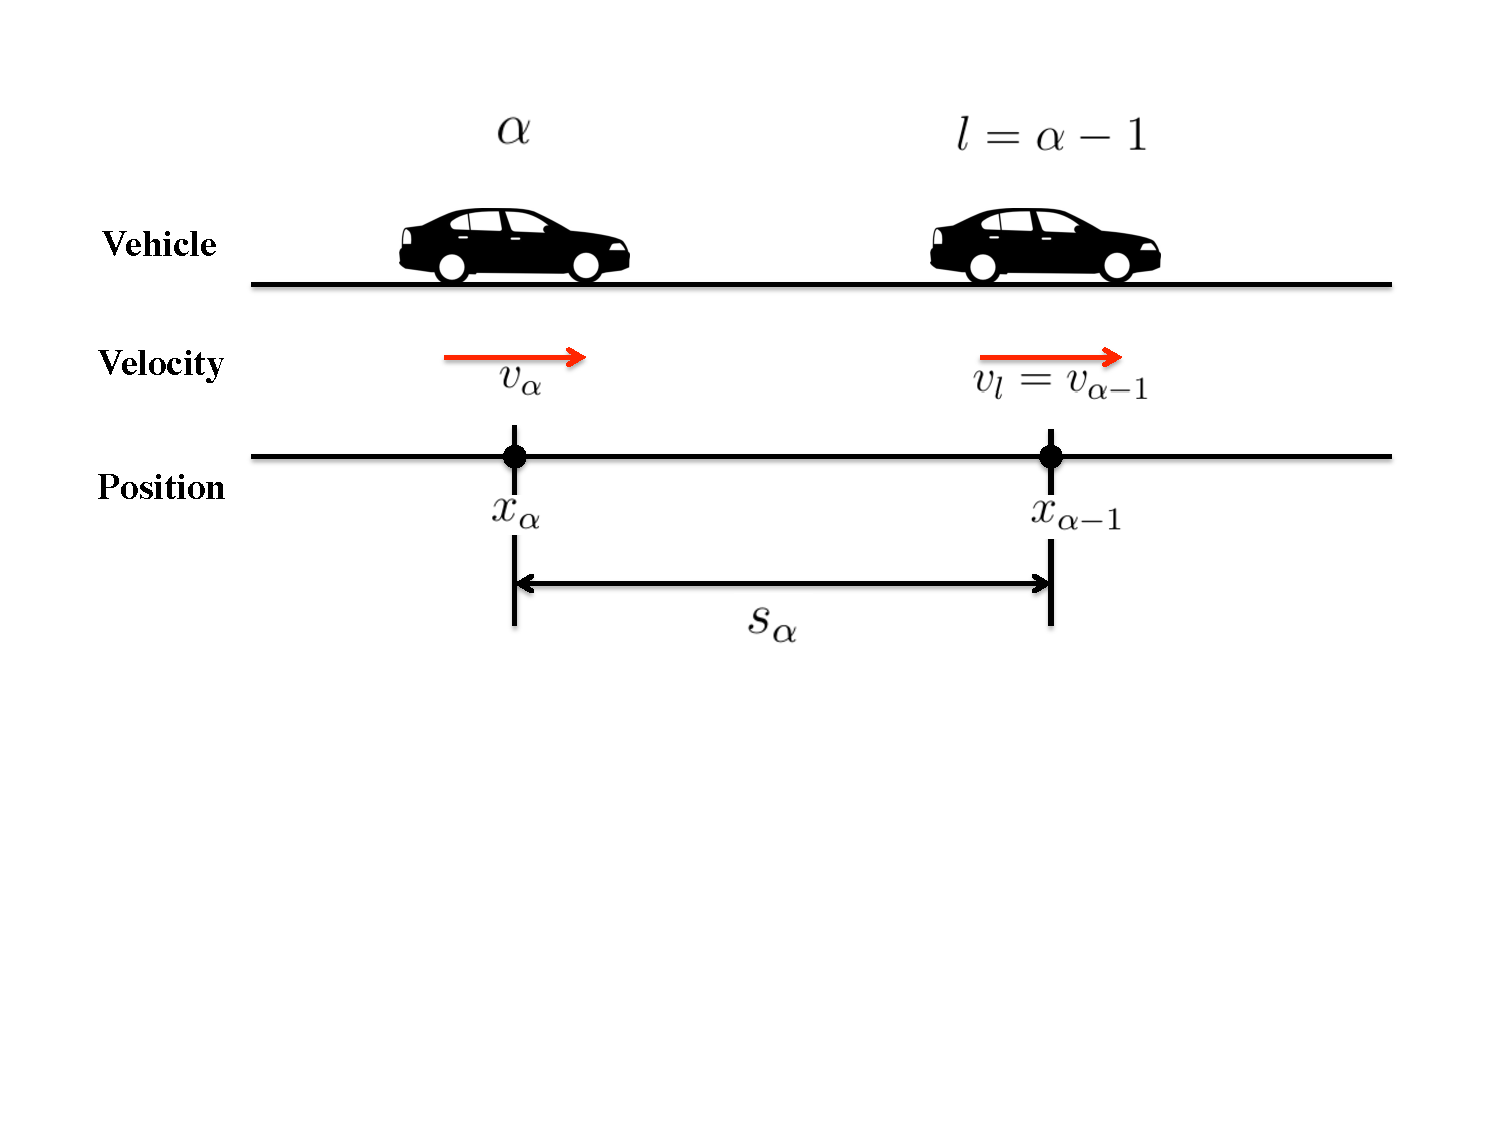
\includegraphics[width=0.95\textwidth]{../figures/system_ppt_fig}}
  \caption{Snapshot of two cars in a system modeled using a car-following model.  The leading car with respect to vehicle $\alpha$  is referred to as vehicle $l=\alpha-1$.  Note that vehicles are represented as particles, and therefore, the vehicles themselves have negligible length.}
\end{figure}
\paragraph{}
The IDM is a simple, accident-free model that can model traffic systems under all realistic traffic conditions.  The acceleration function, shown in Eq (1), of a particular vehicle $\alpha$ is a function the current gap between itself and the leading vehicle ($s_\alpha$), the desired speed $v_0$, and the speed of the vehicle leading vehicle $v_l$.  

\begin{mymathbox}[title=IDM Parameters, colframe=blue!30!black]
  \begin{itemize}
    \item $a$: maximum acceleration
    \item $b$: maximum comfortable deceleration
    \item $s_0$: minimum bumper-to-bumper gap (between vehicle and leading vehicle)
    \item $v_0$: desired speed
    \item $T$: minimum time gap (between vehicle and leading vehicle)
    \item $\delta$: acceleration exponent
  \end{itemize}
\end{mymathbox}

\begin{mymathbox}[ams gather, title=IDM Governing Equations, colframe=blue!30!black]
  \begin{align}
  \dot{v}_\alpha &= a \left[1 - \left(\frac{v_\alpha}{v_0}\right)^{\delta} - \left(\frac{s^*(v_\alpha,\Delta v_\alpha)}{s_\alpha}\right)^{2}\right]\\
  s_\alpha &= x_{\alpha-1}-x_\alpha=x_{l}-x_\alpha\\
  \Delta v_\alpha &=v_\alpha-v_{\alpha-1}=v_\alpha-v_l\\
  s^*(v_\alpha, \Delta v_\alpha) &= s_0 + \max\left(0, v_\alpha T + \frac{v_\alpha \Delta v_\alpha}{2 \sqrt{ab}} \right)
  \end{align}
\end{mymathbox}
\paragraph{}
The first term in Eq (1) is the \textit{free acceleration}\---the acceleration that a vehicle would take if on an open road, without considerations of desired speed or gap.  The second term in Eq (1) is the effect on the acceleration of the vehicle approaching its desired speed.  The third term in Eq(1) is the effect on the acceleration of relative difference between the desired gap distance $s^*(v_\alpha,\Delta v_\alpha)$ and the current gap distance.  The desired gap distance given by Eq (4) the sum of two terms the steady state desired safe distance $s_0+v_\alpha T$ and a dynamical term $\frac{v_\alpha \Delta v_\alpha}{2 \sqrt{ab}}$ representing the intelligent vehicle's braking strategy.

\subsubsection{Improved Intelligent Driver Model (IIDM)}
\paragraph{}
The Improved Intelligent Driver Model is an IDM model with an improved acceleration function that aims to correct three unrealistic qualities of the IDM:
\begin{enumerate}
  \item 
  If a vehicle exceeds the desired speed, the IDM acceleration function will return a very large negative acceleration.  This is unrealistic since drivers on a highway tend to oscillate around their desired speed.  
  \item
  If a vehicle is close to the desired speed, the desired gap $s^*(v_\alpha,\Delta v_\alpha)$ becomes much greater than $s_0 + v_\alpha T$.  This causes the gaps between vehicles to be unrealistically large and can preclude vehicles from reaching the desired velocities.
  \item
  If the actual gap is less than the desired gap distance (e.g. when another vehicle merges into the particular vehicle's lane), then the acceleration function will return an excessively large negative acceleration.  This unrealistic as drivers typically brake lightly to increase the gap.
\end{enumerate}
\begin{mymathbox}[ams gather, title=IIDM Governing Functions, colframe=blue!30!black]
  \begin{align}
  \frac{dv_\alpha}{dt}\Bigr|_{v_\alpha\le v_0}&= 
  \begin{cases}
    a (1-z^2) & z_\alpha \ge 1\\
   a_{\text{free},\alpha}(1 - z_\alpha^{(2a)/a_{\text{free},\alpha}})& \text{otherwise}
  \end{cases}
  \\
  \frac{dv_\alpha}{dt}\Bigr|_{v_\alpha> v_0}&= 
  \begin{cases}
    a_{\text{free},\alpha} + a (1-z_\alpha^2) & z_\alpha \ge 1\\
    a_{\text{free},\alpha} & \text{otherwise}
  \end{cases}\\
  a_{\text{free},\alpha}(v_\alpha)&= \begin{cases}
  a \left[ 1 - (\frac{v_\alpha}{v_0})^\delta \right] & v_\alpha \le v_0\\
  -b \left[ 1 - (\frac{v_0}{v_\alpha})^{a\delta/b} \right] & v_\alpha > v_0
  \end{cases}\\
  z_\alpha&= \frac{s^*(v_\alpha, \Delta v_\alpha)}{s_\alpha}
  \end{align}
\end{mymathbox}
\paragraph{}
The IIDM governing equations seek to improve the unrealistic qualities of the IDM model. Eq (8) is the free acceleration equation, which limits the deceleration's magnitude when $v_\alpha>v_0$ to be at most b. To improve the acceleration function near the desired speed, we use $z_\alpha$ to indicate whether the desired gap distance is greater than the current gap distance or not.  When $v_\alpha < v_0$, the IIDM's acceleration function (Eq (5) and Eq (6)) ensures that the actual gap is no larger than the minimum safe gap $s_\alpha = s_0+vT$.  To maintain the intelligent and comfortable brake method of the IDM, the improved acceleration function only changes when the actual gap is near the desired gap or when the actual velocity is greater than the desired velocity.
\subsubsection{Adaptive Cruise Control Model (ACC)}



\paragraph{}
$$a_{CAH}(s,v,v_l, \dot{v}_l)= \begin{cases}
\frac{v^2\tilde{a}_l}{v_l^2 - 2 \tilde(a)_l} & v_l(v-v_l) \le -2s\tilde{a}_l\\
\tilde{a}_l - \frac{(v-v_l)^2 \Theta (v-v_l)}{2s} & otherwise
\end{cases}$$

$$\tilde{a}_l(\dot(v)_l) = min(\dot{v}_l, a)$$

$$a_{ACC}= \begin{cases}
a_{IIDM} & a_{IIDM} \ge a_{CAH}\\
(1-c)a_{IIDM} + c\left[a_{CAH} + b tanh(\frac{a_{IIDM}-a_{CAH}}{b}) \right] & otherwise
\end{cases}$$

$$\dot{v}(t) = a_{mic}\left[s(t-T_r), v(t-T_r), v_l(t-T_r) \right]$$

$$u(t-Tr) = ru_{i-j-1} + (1-r)u_{i-j},  \, \, j = int\left(\frac{T_r}{\Delta t} \right), \, \, r = \frac{T_r}{\Delta t} - j$$

$$ln s^{est} - ln s = V_s w_s(t) $$

$$v^{est} - v_l = -s \sigma_r w_l(t)$$

%This numerical analysis can be contrasted to the analytical solution that was presented in (**another section 2?**).\par
%A car`s speed is governed by the laws of motion:
%\begin{equation}
%v_f = v_i + a\Delta t
%\end{equation}
%
%An individual car can be modeled as such over a 100,000m track and asked to travel at $v_{target} = 60miles.h^{-1}$ (i.e. $26.8m.s^{-1}$). As the driver is not an perfect controller he is unable to hold the speed exactly at $v_{target}$. We can therefore model his fluctuations as random acceleration with the corresponding adjustments to correct the acceleration:
%\begin{equation}
%a_{correction_i} = \alpha(v_{instant} - v_{target}) + N(0,\sigma_1)
%\end{equation}
%
%We note that for more than one car in a stream of traffic the car's acceleration is then also dependent on the car ahead of it:
%\begin{equation}\label{eq:interaction}
%a_{interaction_i} = \beta (s_{instant} - s_{target})
%\end{equation}
%
%In equation \ref{eq:interaction}, we see that the acceleration of the car is also dependent on the distance between any one car and the car that is directly ahead of it. The final acceleration of the car is therefore:
%\begin{equation}\label{eq:acceleration}
%a_{i} = a_{correction_i} + a_{interaction_i}
%\end{equation}
%
%If we assume the cars should travel at $v_{target}$ and that they should maintain an $s_{target} = 5m$ spacing between them, we can then model the velocity of the car as:
%
%\begin{equation}\label{eq:velocity}
%v_{i} = \frac{d(a_i)}{dt}
%\end{equation}

\section{Microscopic Perspective of Traffic Interaction : Human Driver Models}

\section{Numerical Simulations of Traffic Systems}

\paragraph{}To generate numerical simulations of Traffic Systems, we first consider the case of 50 cars on a circular track. We explored scenarios of all IDM cars and all HDM cars. Under these conditions, we see the IDM models generate more `phantom` traffic waves than the HDM models, especially for larger numbers of HDM car lookahead. This is because the human drivers tend to appear more conservative in a situation like this, with no external perturbations, as the multi-car lookahead prevents them from getting overly close to the car directly in front of them.

% \begin{figure}[H]
% \centering
% \includegraphics[keepaspectratio=true,scale=0.6]{problem3d}
% \caption{Plot of temperature cross section in pipe at various time-steps of simulation}\label{visina8}
% \end{figure}

% \begin{figure}[H]
% \centering
% \includegraphics[keepaspectratio=true,scale=0.6]{problem3d}
% \caption{Plot of temperature cross section in pipe at various time-steps of simulation}\label{visina8}
% \end{figure}

\paragraph{}We then moved on to simulations of a platoon of cars with some cars being controlled by IDM-type models (in particular, Adaptive Cruise Control) and some cars being controlled by multi-car lookahead HDM models. After allowing the models to run for some time to develop their natural spacing, we then perturbed the acceleration of the lead car, causing it to brake and then resume again. We then observe both the magnitude and length of the volatility of the velocities in the following cars after the event. We find that in general, as one would expect, a larger proportion of IDM-controlled vehicles results in a quicker dissipation of the perturbation as well as a lowered probability of a vehicle collision.\\
\textbf{RESULTS HERE}

\section{Stability and Error Comparison of a Variety of Numerical Integration Schemes}
Because there is no analytical solution given for our highly-nonlinear problem, to analyze the error of our numerical integration schemes, we compared to the python \texttt{odeint} solver function. For large enough time steps, this shows us error decreasing on a log scale for each of our higher order methods. However, for small time steps, the `error` for 4th and 5th order methods converges, as the \texttt{odeint} solver presumably decides that 4th order is sufficiently accurate at these time steps and stops using higher order methods.\\
\textbf{RESULTS HERE}
\paragraph{}For our purposes, we desired to use higher order methods such that we could use larger timesteps and hopefully decrease running time of our programs while still maintaining stability in the differential equation systems. To display the effectiveness of these higher order methods, we ran one of our simple models for a variety of time steps over the same total time with the different solvers and noted the number of time steps at which each method stabilized.\\
\textbf{RESULTS HERE}

\section{String Stability of Traffic Systems to Perturbation}

%as a function of the reaction time Tr and the attention span ?t depends strongly on
%the number of considered vehicles. When considering na = 5 leaders, the critical
%effective reaction time Tr + ?t/2 at the stability limit is about twice as large as
%the corresponding critical value without multi-anticipation (na = 1). Particularly,
%traffic can be stable even if the reaction time exceeds the average time headway. This
%agrees with everyday observations but cannot be realized in simulations without
%multi-anticipation. There are limits, however: Anticipating more than five vehicles
%ahead will change the dynamics insignificantly

\section{Optimization of Traffic Systems}
\paragraph{}We set up a number of optimization programs to attempt to search for the optimal values of some of the many parameters for the system as a whole and for individual drivers for a number of cost functions, including maximizing displacement and maximizing comfort (minimizing jerk). The initial trials for these systems were run on IDM models, and the results are largely what one would suspect. When attempting to maximize total displacement, the cars drive quickly and close together, resulting in the creation of traffic waves in the system. When attempting to minimize jerk, the cars drive much more conservatively, as one would expect, never coming within the range of another car that would cause them to change acceleration. \\
\textbf{RESULTS HERE}
\paragraph{}We then attempted to optimize behavior for a single driver and were interested to see what implications this would have for the system as a whole. However, unsurprisingly, the following behaviors in the IDM are such that a single driver can tailgate and maximize target speed basically as much as we will allow without ever disrupting the rest of the system. Even when adding some stochasticity to the lead car, we were unable to see the rest of the system suffer from traffic waves due to the behavior of the second car, because that behavior would simply be quickly dissipated by the third car. In fact, it seems to be true generally of these systems that unless the aggressive driving behavior of a car causes other cars to collide behind it, the greater distance achieved by one car inevitably results in other cars also achieving a greater distance/average velocity. However, this is likely to occur with much greater volatility in the velocity of the cars, i.e. a less pleasant ride. Then, to quantify how the erratic driving of a single car may result in penalties to the system as a whole but not to that car, we must analyze the cost to the other cars in terms of the volatility of their ride speed and possible collisions.\\
\textbf{RESULTS HERE}
\paragraph{}Next, we attempted to replicate these experiments with the more complicated Human Driver Model. However, due to the highly piecewise nature of the functions we are attempting to optimize over, we were unable to use traditional minimization solvers. Instead, we discretized the parameter space we were interested in exploring and searched for the set of parameters which would minimize our target cost function. \\
\textbf{RESULTS HERE}
\section{TODO}
develop a cost function for emissions/energy usage and optimize over that \\
can we find the parameters that will cause a phantom traffic jam?



\section{Traffic Flow Simulation: Microscopic models}

\section{Models and Methods}

\section{Results}

\section{Discussion}

\section{Conclusion}



% Your references go at the end of the main text, and before the
% figures.  For this document we've used BibTeX, the .bib file
% scibib.bib, and the .bst file Science.bst.  The package scicite.sty
% was included to format the reference numbers according to *Science*
% style.


\bibliography{scibib}

\bibliographystyle{Science}



\end{document}




















